% !TeX spellcheck = de_DE
\section{Моделирование посадки ВА}
В результате моделирования были получены графики требуемых траекторий, скоростей и ускорений (показано на рис. ~(\ref{fig:init})), пространственная траектория полета ВА (показано на рис. ~(\ref{fig:3d_traj})), требуемой траектории по высота и требуемой траектории по высоте с учетом модального управления (показано на рис. ~(\ref{fig:high})), отклонения от требумой траектории с учетом управления (показано на рис. ~(\ref{fig:error})).
\begin{figure}[h]
	\centering
	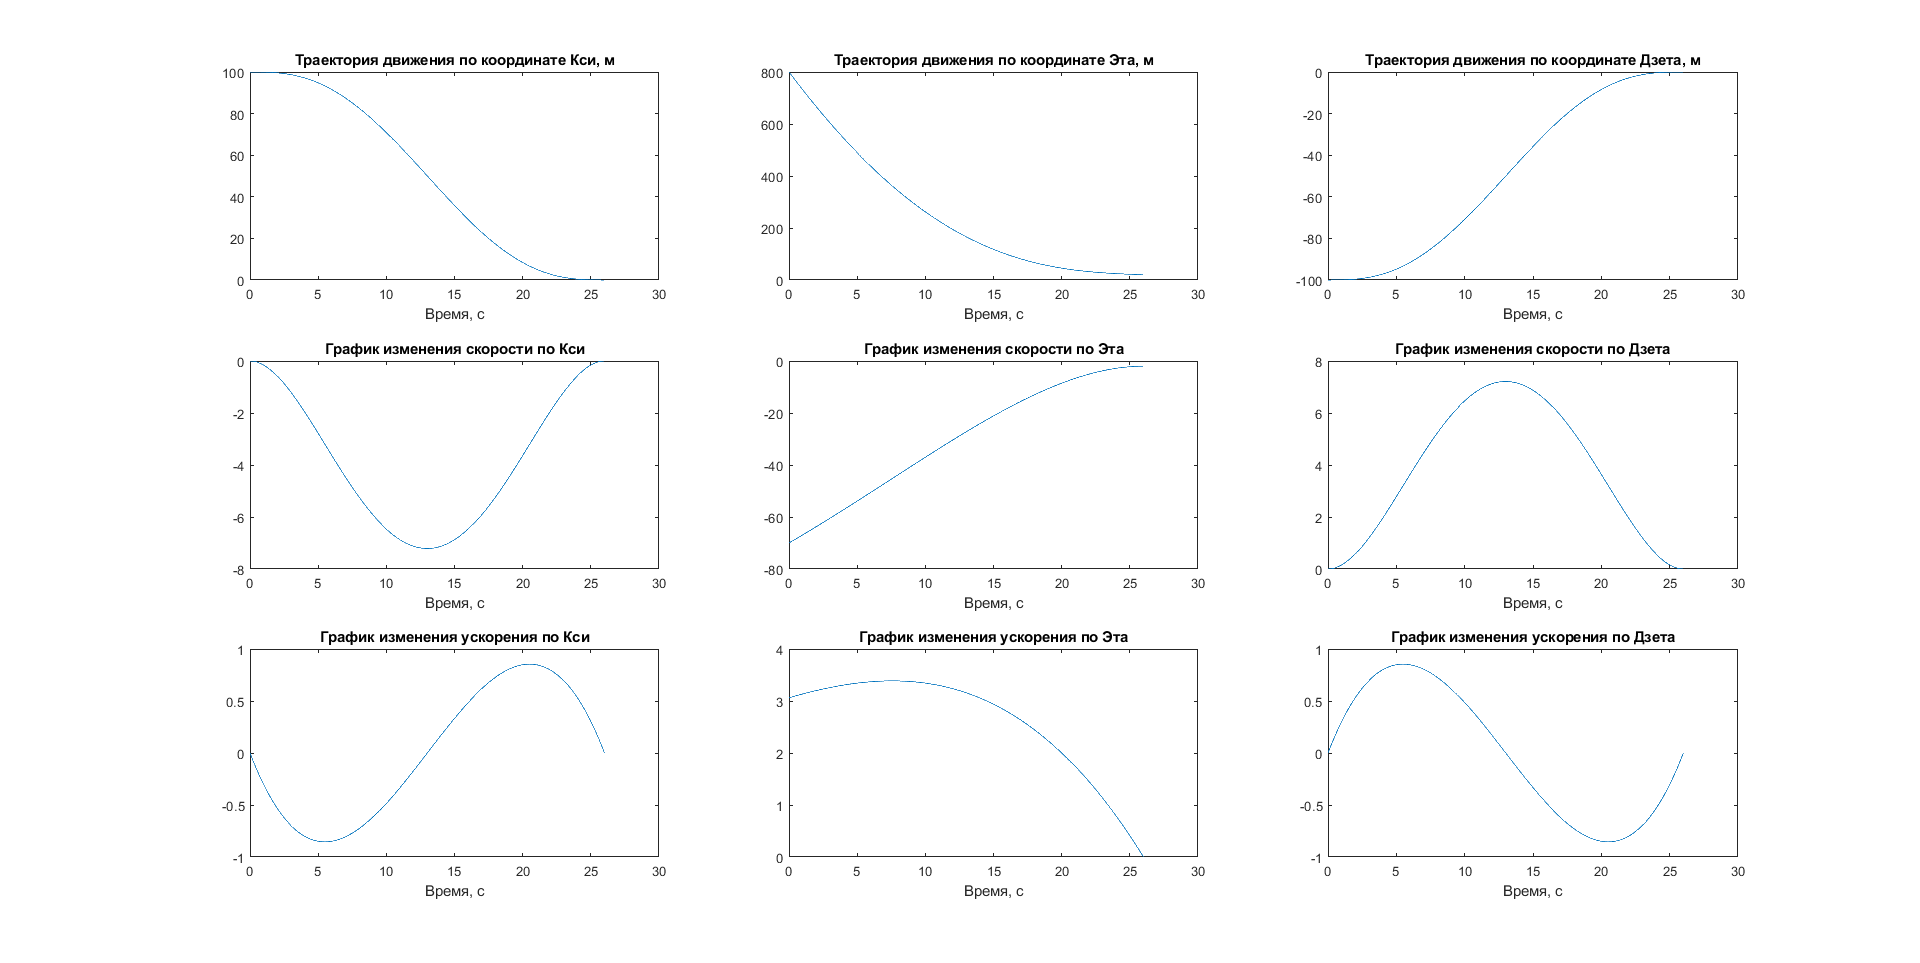
\includegraphics[scale=0.36]{images/path_speed_boost.png}
	\caption{Графики требуемых траекторий, скорости и ускорений}
	\label{fig:init}
\end{figure}

\begin{figure}
	\centering
	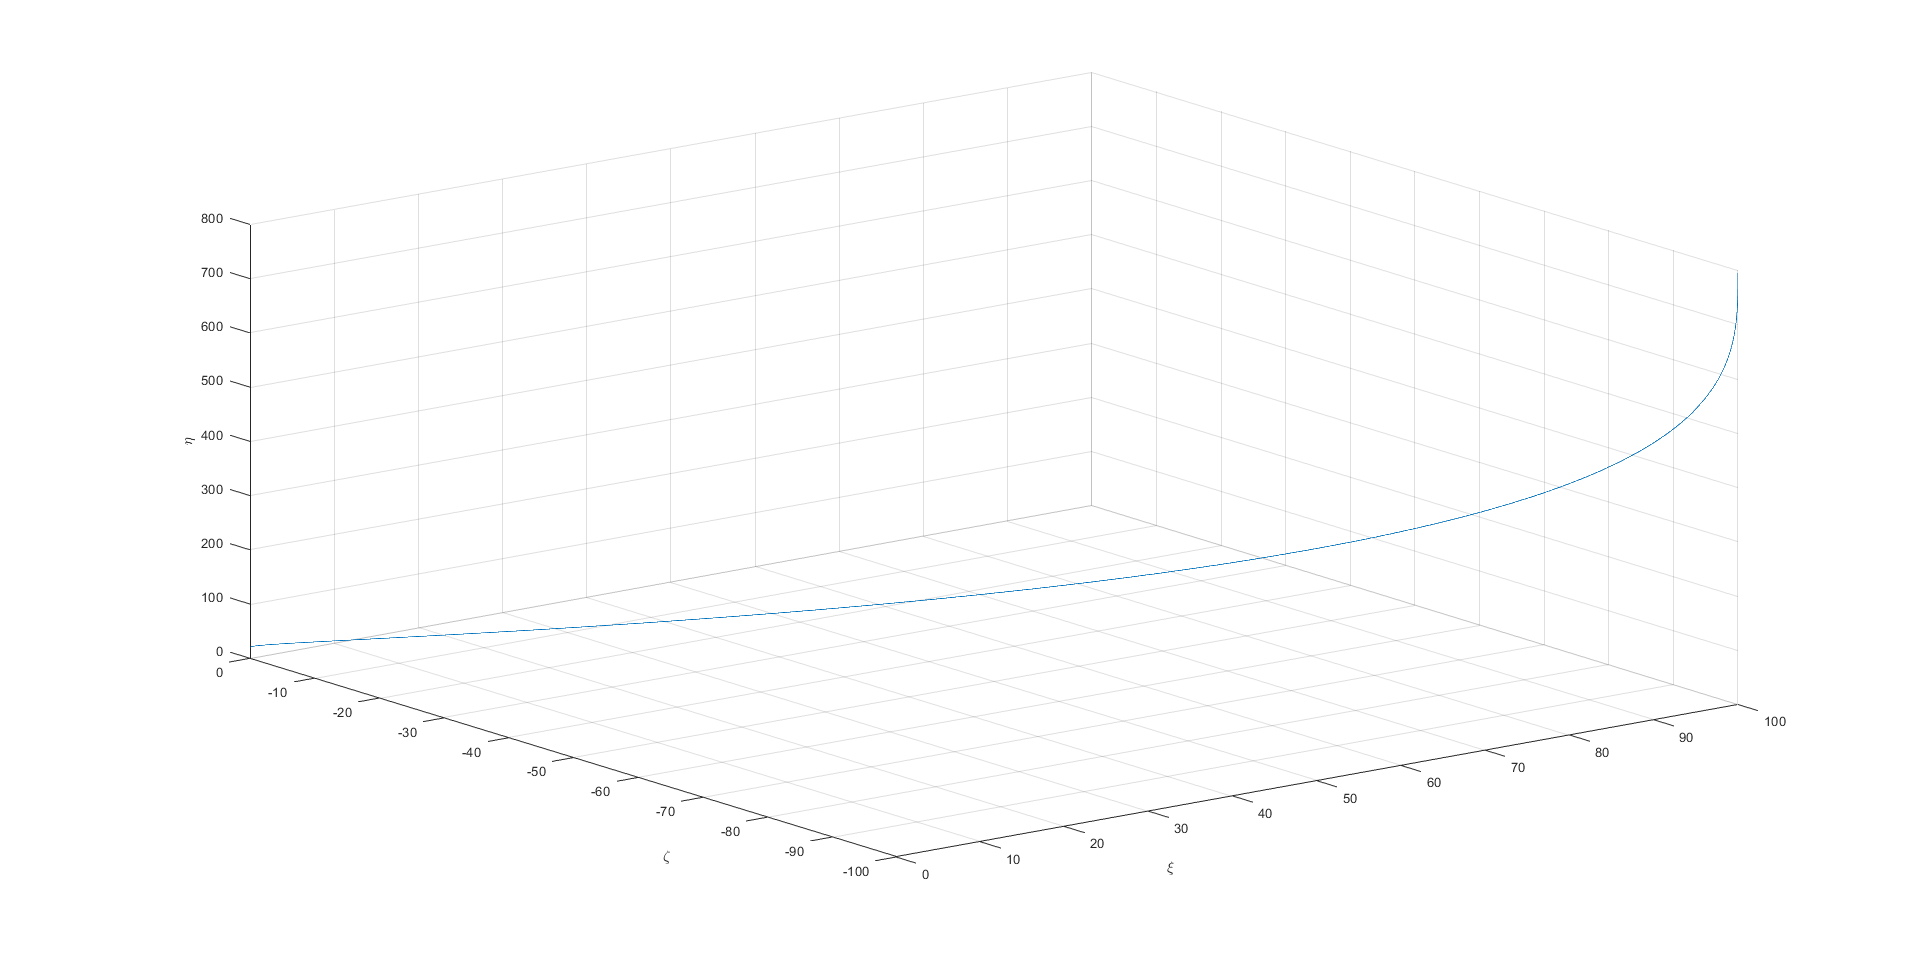
\includegraphics[scale=0.3]{images/3d_traj.png}
	\caption{Пространственная траектория полета ВА}
	\label{fig:3d_traj}
\end{figure}
\begin{figure}
	\centering
	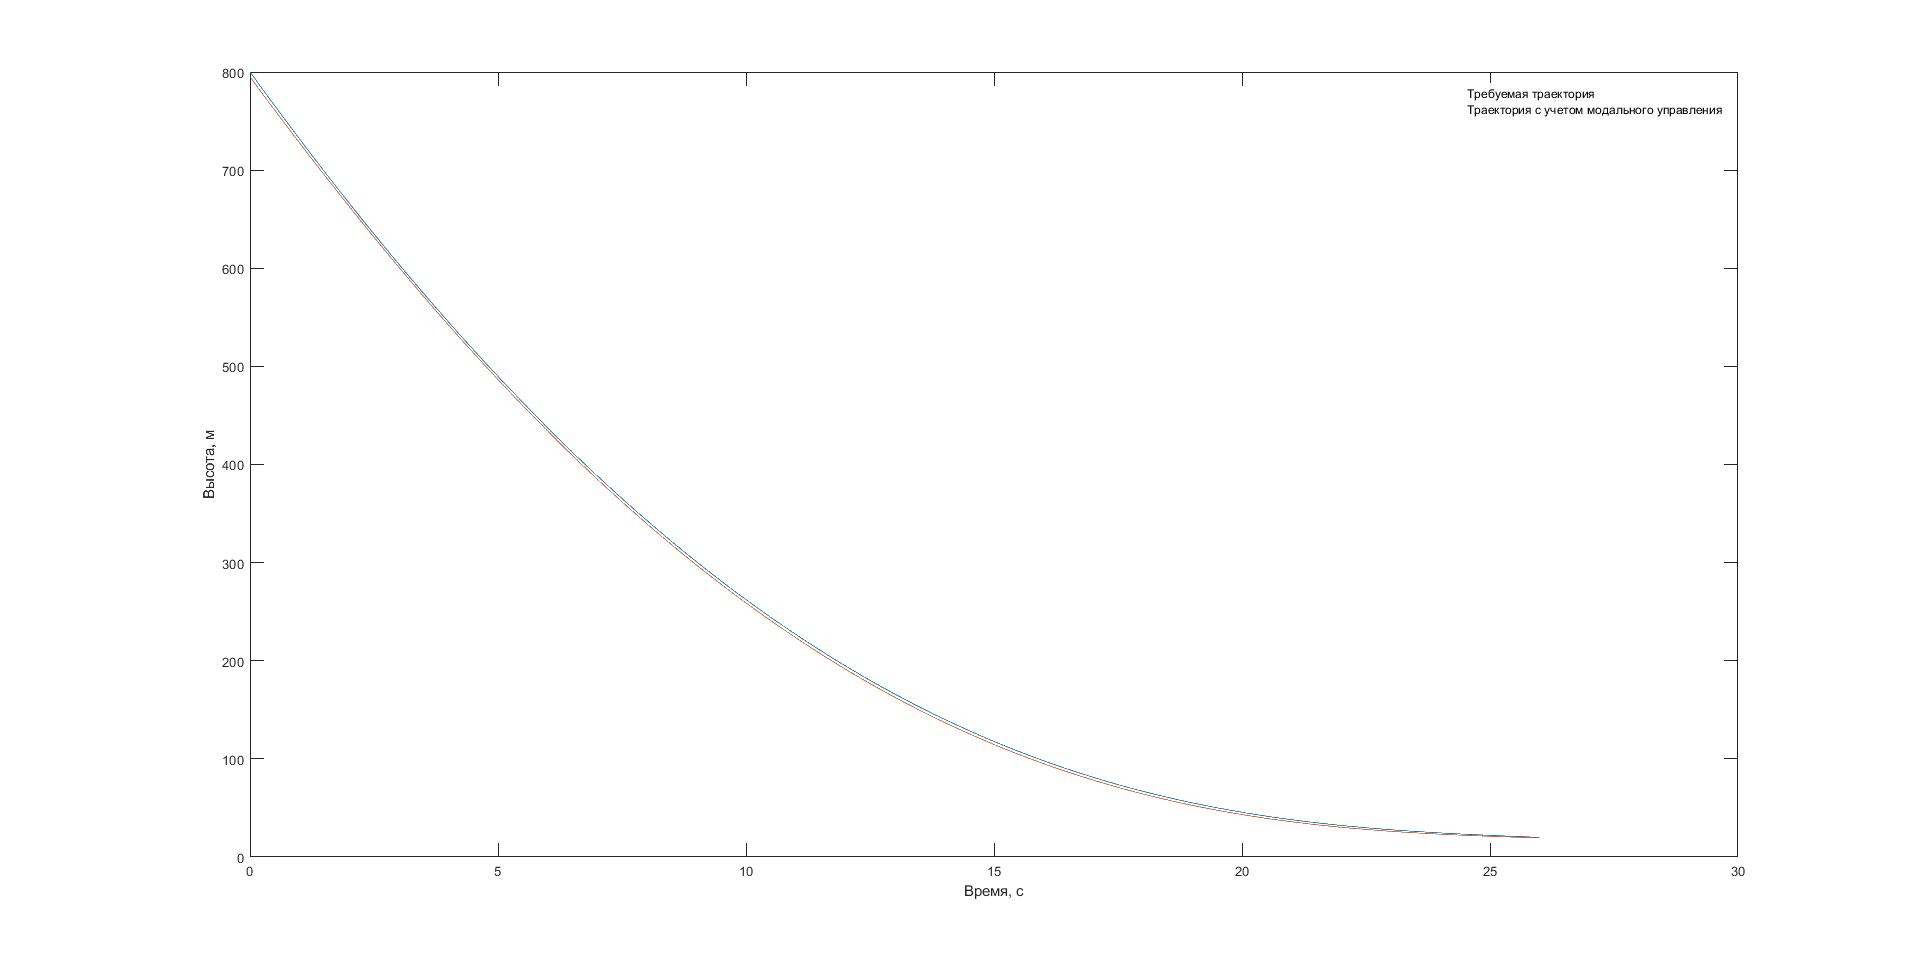
\includegraphics[scale=0.3]{images/pathBias.png}
	\caption{Изменение высоты ВА с учетом  модального управления и требуемое изменение высоты ВА}
	\label{fig:high}
\end{figure}

\begin{figure}
	\centering
	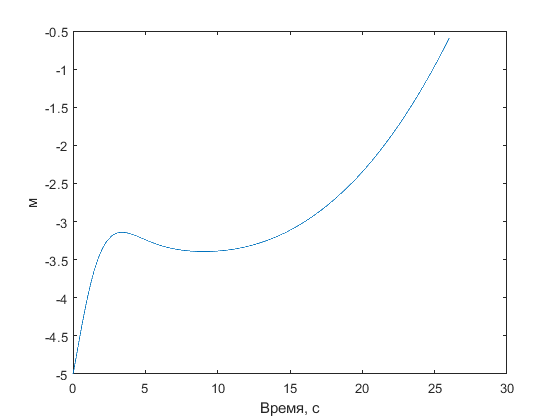
\includegraphics[scale=0.6]{images/error.png}
	\caption{Отклонение от требуемой траектории с учетом управления}
	\label{fig:error}
\end{figure}
\clearpage